


\chapter{Feline High-Rise Syndrome}


\begin{marginfigure}
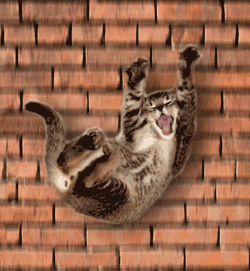
\includegraphics[width=5cm]{figs/CatFall}
\caption{An adorable image of a falling cat, from {\em{http://finickymeterisnotavailable.blogspot.com}}}
\end{marginfigure}

\newthought{It is often said} that cats ``have nine lives''; it is at least a common belief that cats are able to survive falls 
from heights that would kill a human.  Certainly there anecdotal evidence that this is true.
%\sidenote{Of course, there is also anecdotal evidence that Elvis is alive.}  
But is it {\it really} true?  If a cat fell out of an upper floor of the Empire State Building, or the Hancock Tower, would it really be able to walk away?  These are the kinds of questions that surely keep you awake at night.

%\section{A physical system, an implicit mental model, and a prediciton}

Unless you happen to have listened to the RadioLab program addressing this topic, your likely response to the questions above is, ``Of course the cat will die!  It's the Empire State Building, for Pete's sake!''.\sidenote{Well, maybe you would not invoke Pete's name in vain.}  And if asked to sketch a graph of feline morality as a function of height of fall, you might draw something like this:

\begin{figure}[h!]
\centerline{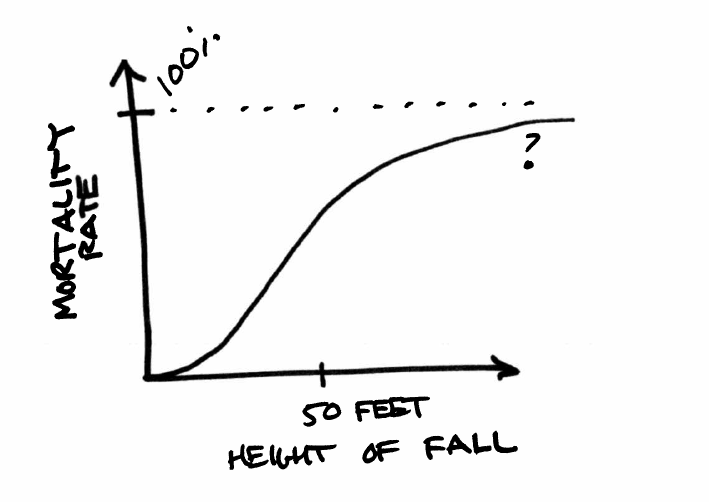
\includegraphics[height=3.5cm]{figs/InitialPrediction}}
\caption{A first prediction about cat mortality as a function of distance fallen. }
\end{figure}


This sketch says that, for relatively short falls, most cats survive -- but above some decent height (say 80 feet?) the cat's chance of survival is very low indeed.  When you create this graph, you are making a set of {\it predictions} -- and you are making those predictions based not on having thrown cats out of buildings, but rather on your intuition about what the result of such an experiment would be.  In other words, you've made a {\it prediction} based on an {\it implicit mental model}, derived from your understanding of an actual {\it physical system} (consisting of cats and buildings):

\begin{figure}[h!]
\centerline{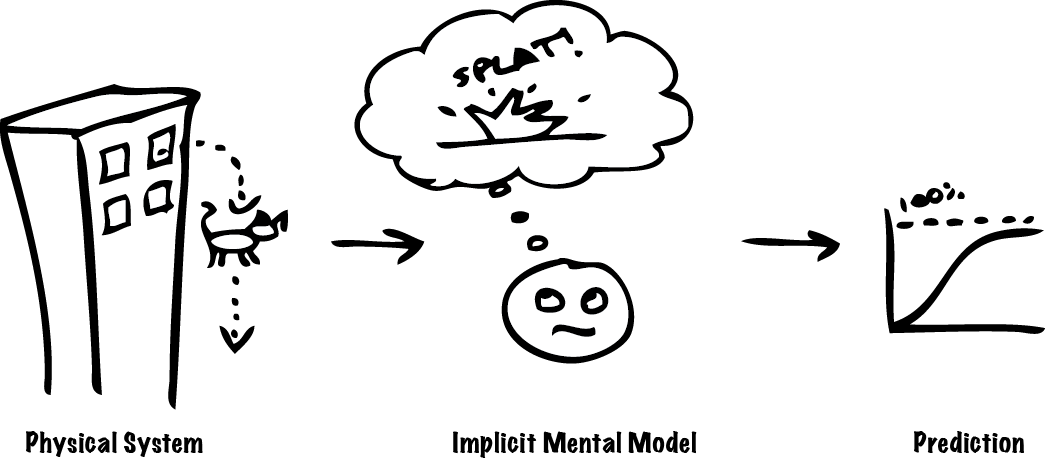
\includegraphics[height=4cm]{figs/SystemImplicitModelPrediction}}
\caption{Cartoon illustrating process of translating a physical system to an implicit mental model, and using that model to make a prediciton.}
\end{figure}


Note that we've made an important distinction here between the actual physical system and our model of the system.  We'll call the process of going from an actual physical system to a model {\it abstraction}, because in doing so, we typically strip away features we think unimportant (e.g., what direction the wind is blowing, or what color the cat is).
\section{Behavior of the physical system}

Of course, if you were particularly enamored of experimentation, or if you found cats particularly distasteful, you might have chosen to skip the thought experiment, and instead try to measure the actual {\it behavior of the physical system}.  While (to my knowledge) only a few sadistic teenagers have ever intentionally thrown cats from great heights, there are veterinarians who have reported the results of accidental feline falls.  Jared Diamond wrote a cute little paper in Nature on this subject 15 years or so ago, and included the figure in the margin showing both injury rates and mortality rates for cats (as well as mortality rates for humans). 
\begin{marginfigure}
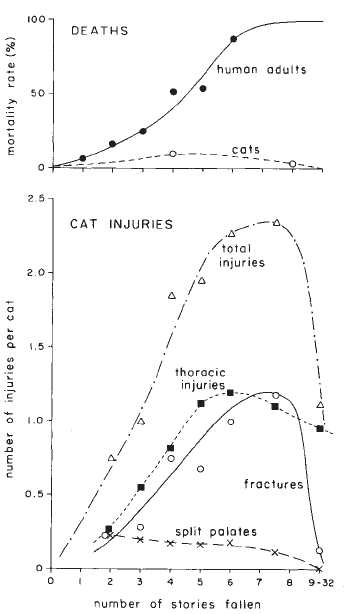
\includegraphics[height=10cm]{figs/DiamondFigure}

\caption{Cat and human mortality and injury rates as a function of height of fall.  From Diamond, {\it Nature}, 332(14), 1988.}
\end{marginfigure}

As can be seen, cats who are brought into the vet's office after falling out of buildings appear to have {\it higher} survival rates when they fall greater distances!  We'll acknowledge here has been a lot of discussion of these results in statistics textbooks and blogs: because only cats that survive get taken to the vets, it's possible that this data suffers from significant sampling bias.  

But whether or not there's a sampling bias here, we do have a problem:  our implicit mental model's predictions seem to be at odds with the observed physical behavior of the system.  It could be that the experiment is faulty; it could be the model is inappropriate; and it's possible that both are problematic.  

\section{Iteration, using physical laws, and doing explanatory work}

Since this is a course on modeling and simulation, let's assume that the observed behavior is reasonably consistent with reality in the entire cat population.
If this is true, then it's pretty clear that the implict mental model that we started out with ("Of course the cat will die!") needs some work.

Just as in design, you often {\it iterate} when modeling -- that is to say, you create a simple ``first draft'' model (or prototype), and you learn some things from that model.  Then you create a second model that improves on the first, and continue the process until you have a model that does what you want it to do.

In this case, it seems like our first pass, implicit mental model doesn't do a good job at all of explaining the observed behavior.  Can we propose something better?

\subsection{A first iteration: a pinch of mechanics}

One obvious option might be to invoke a bit of mechanics.  Upon falling out of a building, a cat will accelerate downwards until the force of gravity is offset by the force of drag, at which point it reaches cat terminal velocity (around 40-60 miles per hour for a cat, depending on the cat's configuration, etc.)  SImilarly, a person will accelerate downwards until he/she reaches human terminal velocity (about 120 miles per hour).  If we try to make a sketch of what the speeds of the cat and the person would look like, we pretty quickly come to a prediction that looks something like this:

\begin{figure}
\centerline{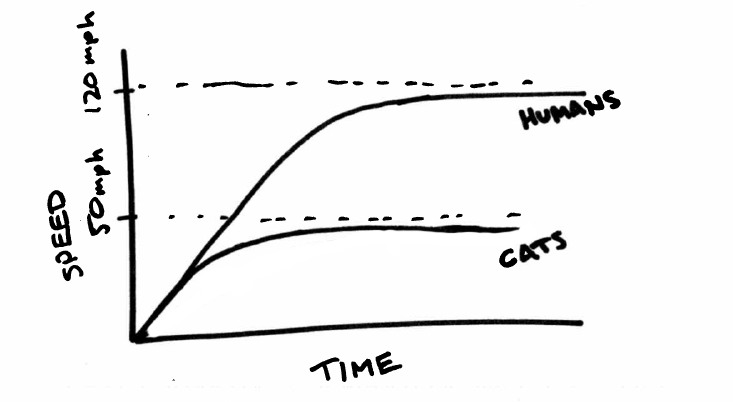
\includegraphics[height=5cm]{figs/TerminalVelocitySketch}}
\caption{Sketch of expected velocity versus distance fallen for humans and cats}
\end{figure}

Here we can see that both the human and the cat initially accelerate at the same rate, but that the cat's speed plateaus much sooner and lower than that of the human.  Note that this immediately suggests at least a partial explanation for why cat mortality rates are so much lower than human mortality:  maybe cats can survive hitting the ground at 40 miles per hour, where as humans aren't so good at surviving a hit at 120.

\subsection{A second iteration: getting more quantitative}
\begin{marginfigure}
\centerline{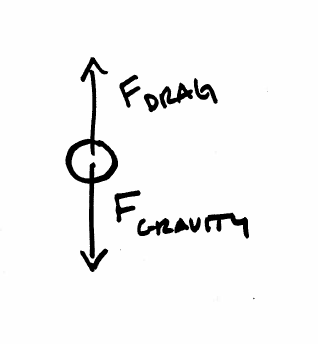
\includegraphics[height=5cm]{figs/CatFBD}}
\caption{Simple free-body diagram for body falling with drag}
\end{marginfigure}
Of course, we can be more formal than just sketching what we think will happen:  we can abstract the cat (or person) to a simpler mechanical system, and then develop equations that describe the behavior of that system.  To do so, we might might start with a free-body diagram of the cat or person,
indicating that the only two important forces acting on a falling person or cat are gravity and drag.

We'd then do some research into drag forces, and invoke Newton's laws to come up with a mathematical model that looks something like this:
$$ \frac{dv}{dt} = g - \frac{1}{2m} C_D \rho A v^2$$
where $v$ is the speed of the falling person or cat, $g$ is the gravitational acceleration, $m$ is the mass of the falling cat/person, $C_D$ is the drag coefficient of the falling cat/person, $A$ is the cross-sectional area of the person or cat, and $\rho$ is the mass density of the atmosphere.  Don't worry right now if this mathematical model is not something you've seen before -- you'll be learning to deal with {\it differential equations} like this later in the semester.  

With this equation, we can either write a simple computer simulation, or do some analytical work, to predict the speed and the position of both the cat and the human as they fall.  A simulation of this equation, using appropriate parameter values for cats and for humans, allows us to create a plot of speed as a function of height of fall:

\begin{figure}

\centerline{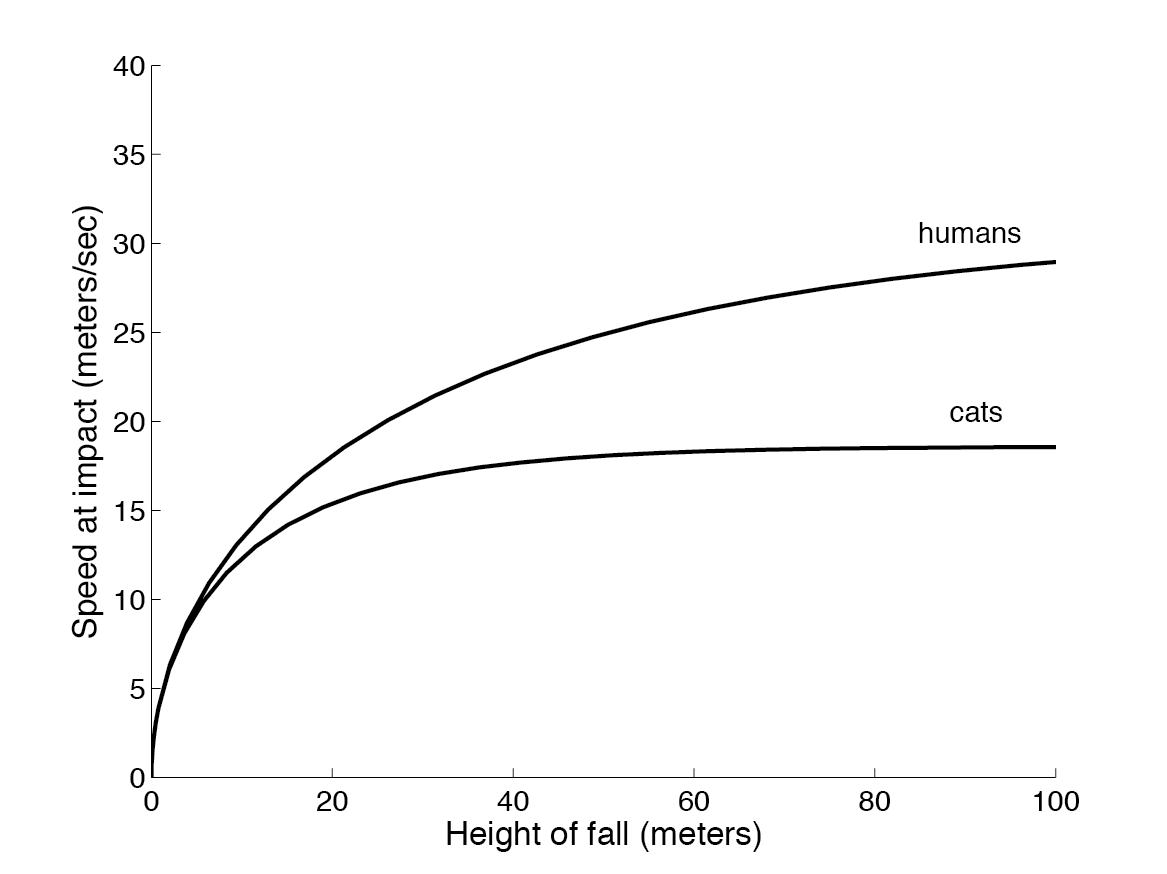
\includegraphics[height=7cm]{figs/CatSpeed}}
\caption{Simulated cat and human velocity as a function of distance fallen.  Note that due to the cat's lower higher area:mass ratio, the cat reaches a lower terminal velocity. }

\end{figure}

Note that we've changed units here from miles per hour and stories to meters per second and meters.  While miles per hour are handy for our intuition, once we get into simulation work it is often a good idea to stick with standard units.  In any case, we are now starting to get a more substantial bit of insight from the model.  The speed of the cat stops increasing somewhere around 20 meters (5 stories): regardless of whether the cat drops 5 stories or 20 stories, it will hit the ground at around 15 or so meters per second.  Humans, on the other hand, hit the ground at a higher velocity than cats -- particularly for falls above 5 or so stories -- and continue to accelerate for a much longer distance (humans don't reach terminal velocity until around 100 stories!).  Furthermore, to the extent that humans seem to have a reasonable survival rate when hitting the ground at a speed below 20 m/sec, it's not unreasonable to expect cats to be able to survive a similar impact.\sidenote{Presumably there is less sampling error associated with human high-rise syndrome.}  

\subsection{A third iteration}

Of course, this model doesn't explain why the mortality rate {\it drops} when the cat falls from greater heights.  Diamond and others speculate that this might be due to an observed difference in cat behavior for shorter versus longer falls.  In a short fall, the cat will tend to try to land on its feet (as you probably know, cats have an impressive ``righting reflex'' that allows them to twist in mid-air and land on their feet).  On the other hand, when cats fall greater distances, they tend to assume more of a ``flying squirrel'' posture.  

We could incorporate this into the model by assuming that the cat's cross-sectional area, and/or drag coefficient, increase after the cat has fallen some distance.
Given the data, it's not unreasonable to guess that this transition might be around 5-7 stories.  If we incorporate this additional feature into the model, we obtain the following simulation results:

\begin{figure}

\centerline{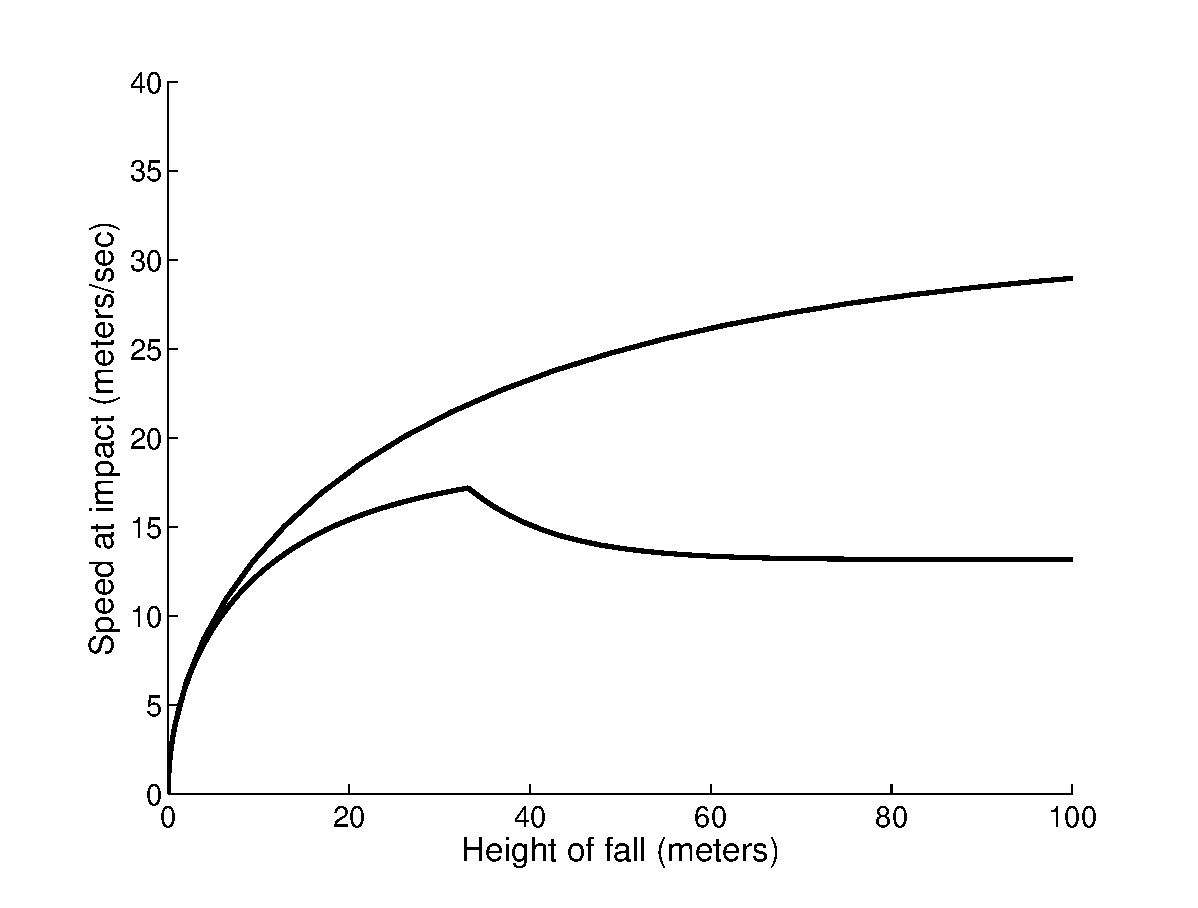
\includegraphics[height=7cm]{figs/CatSpeedWithPosture}}

\caption{Simulated cat and human velocity as a function of distance fallen, with an assumed change in drag coefficient and cross-sectional area for the cat at 35 meters. }

\end{figure}



Here we can see that the cat's peak speed occurs just before it spreads its legs into the flying squirrel position, and that the cat then slows down, hitting the ground at lower speeds for greater heights.  This could help partially to explain why cats have better survival rates, and lower injury rates for falls from greater heights.  We could imagine other reasons why the ``flying squirrel'' position might be beneficial.  For example, the impact is spread out over a larger area, resulting in a smaller impulse per unit area when the cat hits the ground.  Similarly, the cat might be more relaxed in this position, and this might result in reduced damage as well (Note the implicit mental models here for damage that we have introduced!).

At this point we certainly don't have a model that tells us mortality rates as a function of height.  But we {\it do} have a physically-based model that can help us to {\it explain} the observed behavior.  In other words, we are able to {\it do work} with this model.  Furthermore, the model allows us to {\it make predictions} that are not covered by the observed behavior:  it seems pretty clear, from the model, that we would expect reasonable cat survival rates even if the cat was doing parachute-free skydiving.  

\subsection{Are we done yet?}

We could, of course, push this further by iterating more.  Maybe we could develop a model for mortality as a function of impact speed (and body mass!).  Maybe we could do a better job of capturing the nuances of how the cat's posture and orientation changes.  But we should question whether such additional steps will add much value:  we have a simple model that does a pretty good job of explaining the behavior, and predicting behavior that we can't (or at least from a moral perspective shouldn't) observe.  And while the model has some stuff that I've made up (particularly around the question of how configuration change effects drag coefficient), it is pretty defensible.  Adding complexity to the model might make it match the data better -- but it certainly would take additional work, and also could diminish the model's credibility if the additions were not well-justified.

\section{A general framework for modeling}

\begin{figure}

\centerline{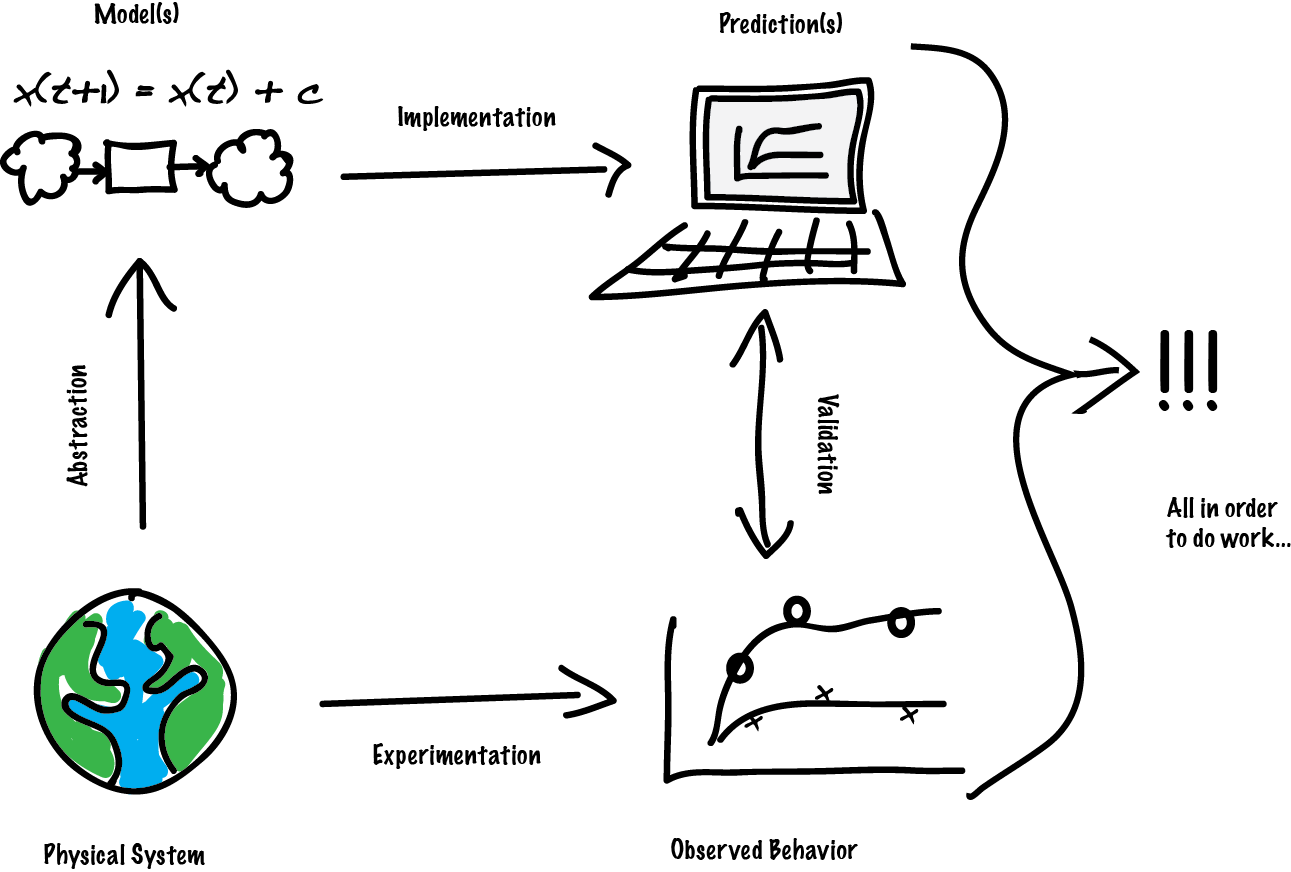
\includegraphics[height=7cm]{figs/LabeledModsimDiagram}}

\caption{Cartoon illustrating the modeling and simulation process}
\end{figure}

The feline high-rise syndrome example we have been discussing is intended to introduce you to a general framework for modeling that we'll be using throughout the course.  The cartoon illustrates this framework. Typically in modeling we start in the physical world, with some {\it physical system} that we want to know about (e.g., cats falling out of buildings).  We then go through a process of {\it abstracting} this system to a {\it model}.  Using the model, we somehow {\it implement} the model to {\it make predictions} -- perhaps by implementing the model as a simulation, perhaps by ``playing the movie in our heads'', perhaps by doing analysis on a set of equations.  With a prediction in hand, we attempt to {\it validate} our model by comparing those predictions with the {\it observed behavior} of the system. 

Importantly, in modeling we almost always go through this cycle multiple times -- just as we did with the cat example.  This iteration is driven by the desire to create a model which {\it does work}.   

In the context of modeling, we think about a number of different, but related, types of work.  {\it Explanatory} work involves helping us to understand an observed phenomenon.  A model does {\it predictive} work if it allow us to say something about an phenomenon that we have not yet directly observed -- e.g., what might happen if a cat jumped out of an airplane.  {\it Design} work is often an extension of predictive work -- e.g., a model might allow us to choose parameters that optimize the performance of a system.

Finally, it is worth noting that iteration in modeling has to stop at some point -- and typically that point is {\it not} when the model is perfectly accurate, but rather is when the model strikes an appropriate balance between simplicity and accuracy for the work that you are trying to do.  Deciding when to continue iterating, and when to stop, requires judgement, which we hope you will develop through this semester, as well as through the rest of your time at Olin.

